\chapter{Problem 1 --- Yang Pulang Membawa Laptopnya}

\section{Identifikasi masalah (butir ``Di laporan'' 1)}

{\small
\begin{longtable}{@{}>{\raggedright\arraybackslash}p{0.405\linewidth}>{\raggedright\arraybackslash}p{0.541\linewidth}@{}}
\toprule
\textbf{Persoalan} & \textbf{Nama dan konsep dalam literatur} \\
\midrule
\endhead
Data tidak muat di satu penyimpanan dan harus dibagi & \textbf{Partitioning / sharding} (Kleppmann, \emph{DDIA} bab 6): setiap record punya tepat satu partisi pemilik. \\
Gempa terkonsentrasi di satu jalur sehingga satu mesin bekerja keras & \textbf{Data skew} dan \textbf{hot spot / hot partition}. Partisi menurut kunci yang berkorelasi dengan wilayah atau waktu menumpuk beban di satu partisi. \\
Laptop pulang membawa sebagian catatan & \textbf{Replication} untuk \emph{durability} dan \emph{availability}: \emph{single-leader (primary--backup) replication} dengan \emph{synchronous standby}, \textbf{failover}, dan bahaya \textbf{split-brain}. \\
Laptop baru harus masuk tanpa mematikan sistem & \textbf{Rebalancing}: memindahkan salinan dan peran primary ke node baru secara online (\emph{re-replication}, \emph{planned switchover}). \\
Membaca lintas lokasi selama sebagian unit hilang & \textbf{Scatter--gather} dengan batas waktu per unit; \textbf{degraded / partial results} (\emph{harvest vs yield}, Fox \& Brewer 1999); trade-off konsistensi--ketersediaan (\textbf{CAP/PACELC}). \\
\bottomrule
\end{longtable}
}

\section{Mekanisme yang dipilih (butir ``Di laporan'' 2)}

\begin{figure}[H]\centering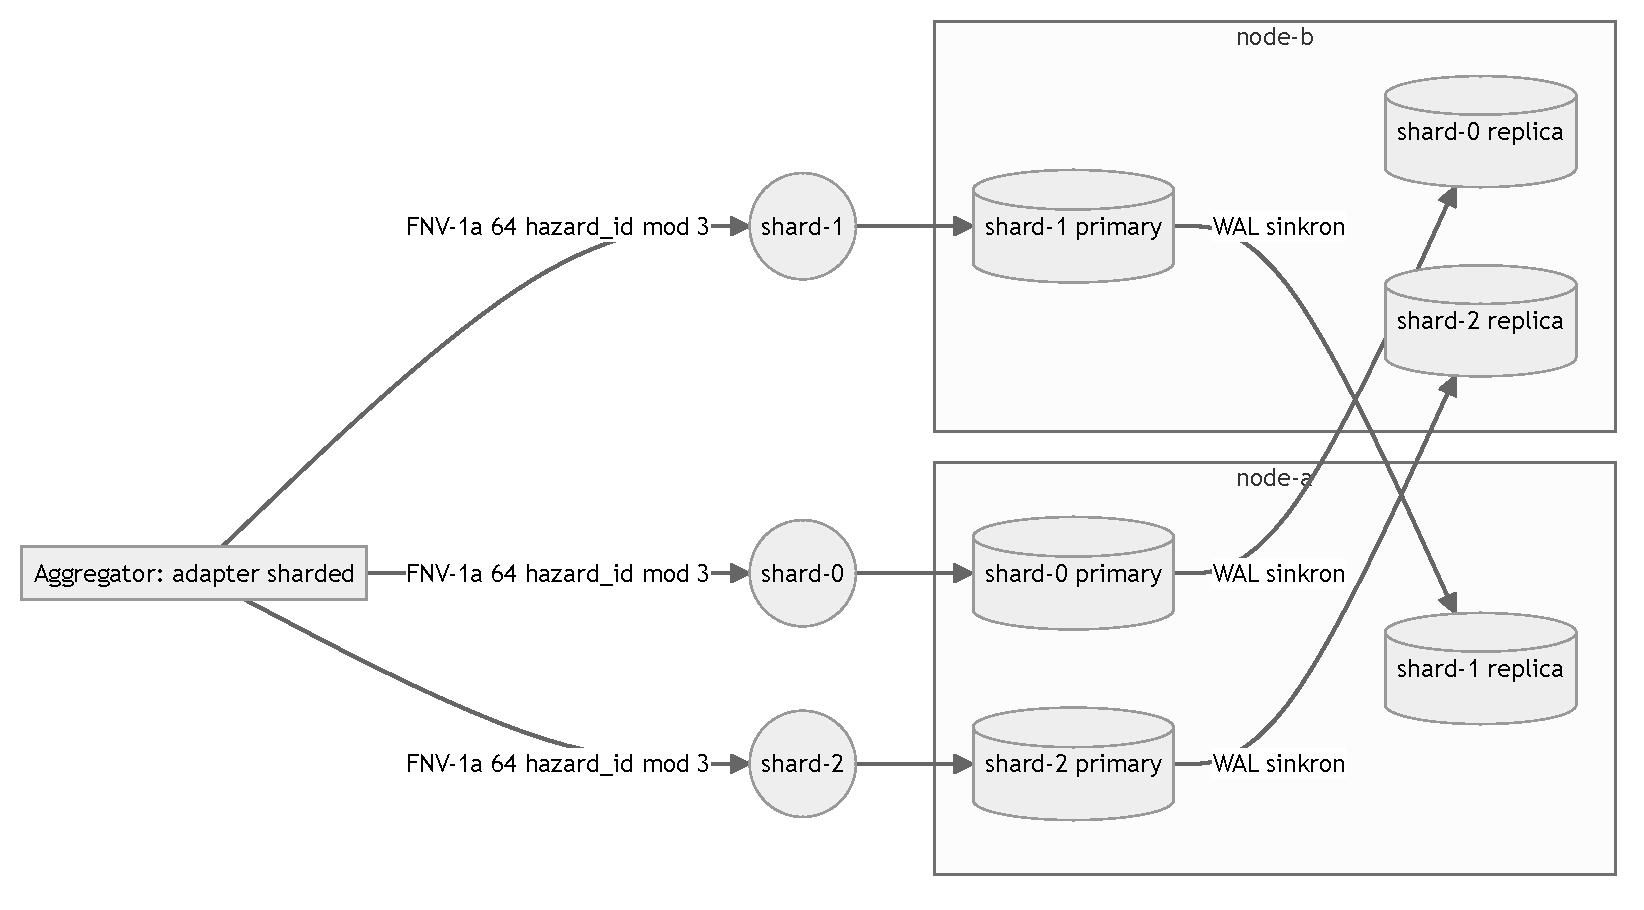
\includegraphics[width=\linewidth,height=0.82\textheight,keepaspectratio]{fig/m3.pdf}\end{figure}

\textbf{Unit penyimpanan.} Canonical Store dibagi menjadi tiga shard logis. Setiap shard adalah satu grup Patroni dengan dua anggota PostgreSQL 16. Kedua anggota berada di node berbeda karena \emph{pod anti-affinity} wajib. Datanya berada di disk node lewat PV \texttt{local-\allowbreak{}path}. Setiap anggota berlabel \texttt{role=\allowbreak{}store}, dengan requests 512Mi dan limits 1Gi (Lampiran B).


\textbf{Di mana sebuah data disimpan.} Aggregator, satu-satunya pemilik store, menghitung \texttt{FNV-\allowbreak{}1a 64(hazard\_\allowbreak{}id) mod 3}. Baris outbox ikut shard hazard-nya dan ditulis dalam transaksi yang sama. Metadata bersama (cursor polling, status sumber, DLQ, checkpoint satelit) berada di shard-0. Shard logis sebuah hazard \textbf{tidak pernah berubah} ketika node datang dan pergi. Yang berpindah hanyalah lokasi fisik salinan dan peran primary. Akibatnya, rebalancing tidak menyalin ulang data antar-shard. Cara ini berbeda dari \emph{consistent hashing} atas node, yang memindahkan kunci saat keanggotaan berubah.


\textbf{Siapa primary.} Patroni menyimpan \emph{leader key} tiap shard di API Kubernetes. Ini sumber kebenaran yang sama dengan lease leader Aggregator pada P2, sehingga keputusan primary tidak bergantung pada jam node. Commit menunggu WAL tersimpan di standby (\texttt{synchronous\_\allowbreak{}mode: true}). Bila primary hilang, standby sinkron yang dipromosikan; salinan usang tidak pernah dipromosikan. Bila standby yang hilang, primary tetap menerima tulis dengan satu salinan (mode sinkron non-strict). Pilihan ini menukar perlindungan terhadap kehilangan \textbf{kedua} selama perbaikan dengan ketersediaan tulis.


\textbf{Sebaran beban tulis.} ConfigMap \texttt{shard-\allowbreak{}placement} menetapkan node pilihan primary tiap shard, dirotasi di node penyimpanan (2 node: shard-0 $\rightarrow$ node-a, shard-1 $\rightarrow$ node-b, shard-2 $\rightarrow$ node-a). \texttt{balance-\allowbreak{}shard} berjalan di setiap anggota dan hanya berbicara dengan API Patroni lokal. Bila leader tidak di node pilihannya, dan anggota di node pilihan sudah \texttt{sync\_\allowbreak{}standby}, \emph{streaming}, lag 0, serta stabil 60 s, leader meminta \textbf{switchover terencana}. Tidak ada data hilang karena kandidatnya sinkron. Ada jeda 300 s antar-switchover untuk mencegah \emph{flapping}. Saat cluster dideploy, ketiga primary mula-mula terpilih di node-b. Satu menit kemudian \texttt{balance-\allowbreak{}shard} memindahkan primary shard-0 dan shard-2 ke node-a tanpa intervensi (log: \texttt{"switchover requested" \ldots{} "Successfully switched over to \textbackslash{}"shard-\allowbreak{}0-\allowbreak{}1\textbackslash{}""}).


\textbf{Ketika node datang dan pergi.}

\begin{itemize}
\item \textbf{Node hilang:} anggota di node lain menjadi primary (failover Patroni). Pembacaan dan tulisan pindah ke sana.
\item \textbf{Node kembali kosong / node baru:} anggota yang PV-nya kosong dibangun ulang otomatis oleh Patroni (\texttt{basebackup} dari primary, lalu \emph{streaming}). Setelah sinkron, \texttt{balance-\allowbreak{}shard} mengembalikan primary ke node pilihan, sehingga node itu ikut menanggung tulisan. Untuk node pengganti bernama lain, \texttt{scripts/\allowbreak{}k8s/\allowbreak{}restore-\allowbreak{}shard.\allowbreak{}sh} memindahkan klaim PV ke node baru.
\item \textbf{Fencing P2 tetap berlaku di setiap shard.} \texttt{RaiseFence} menaikkan term di semua shard, dan setiap tulisan memeriksa fence di transaksinya sendiri.
\end{itemize}

\section{Alternatif dan konsekuensinya pada kriteria 2 (butir ``Di laporan'' 3)}

Ketiga strategi diukur offline pada input yang \textbf{sama} dengan yang dimuat ke cluster: katalog 5.000 gempa dengan kemiringan alami (Sumatera Barat terbanyak) ditambah lonjakan 1.500 gempa di Sumatera Barat. Penempatannya dihitung oleh \texttt{tools/\allowbreak{}catalog/\allowbreak{}catalog.\allowbreak{}py distribution} (\texttt{docs/\allowbreak{}evidence/\allowbreak{}m2/\allowbreak{}p1-\allowbreak{}load-\allowbreak{}latest.\allowbreak{}log} §5).


{\small
\begin{longtable}{@{}>{\raggedright\arraybackslash}p{0.281\linewidth}>{\raggedright\arraybackslash}p{0.191\linewidth}>{\raggedright\arraybackslash}p{0.106\linewidth}>{\raggedright\arraybackslash}p{0.225\linewidth}>{\raggedright\arraybackslash}p{0.106\linewidth}@{}}
\toprule
\textbf{Strategi (3 shard)} & \textbf{Seluruh data: baris per shard} & \textbf{max/mean} & \textbf{Tulisan 24 jam terakhir (lonjakan)} & \textbf{max/mean} \\
\midrule
\endhead
**Hash \texttt{hazard\_\allowbreak{}id} (dipilih)** & 2151 / 2178 / 2171 & \textbf{1,01} & 491 / 509 / 500 & \textbf{1,02} \\
Range per \texttt{area\_\allowbreak{}name} & 1897 / 1298 / 3305 & 1,53 & 0 / 0 / 1500 & 3,00 \\
Range per \texttt{occurred\_\allowbreak{}at} (potongan kuantil) & 2166 / 2167 / 2167 & 1,00 & 0 / 0 / 1500 & 3,00 \\
\bottomrule
\end{longtable}
}

\begin{itemize}
\item \textbf{Range per wilayah:} query per wilayah murah (satu shard), tetapi wilayah teraktif menjadi \emph{hot partition} permanen. Seluruh lonjakan Sumatera Barat jatuh ke satu shard.
\item \textbf{Range per waktu:} seimbang untuk data historis dan \emph{range scan} waktu efisien, tetapi \textbf{semua tulisan baru} selalu menuju partisi terbaru (\emph{write hotspot}).
\item \textbf{Hash (dipilih):} tulisan tersebar rata, termasuk saat lonjakan. Konsekuensinya, setiap query lintas wilayah atau waktu harus \emph{scatter--gather} ke semua shard lalu di-\emph{merge}, dan locality per wilayah hilang.
\end{itemize}

\textbf{Sebaran per node} mengikuti letak primary. Dengan 3 shard di 2 node, node-a memegang 2 primary, sehingga beban tulis terukur 71 \% node-a / 29 \% node-b, baik saat katalog dimuat (+4.099 / +1.700 tulisan) maupun saat lonjakan (+1.244 / +519). Ketidakseimbangan ini disebabkan jumlah shard yang tidak habis dibagi jumlah node, bukan oleh kemiringan data. Dengan 3 node, atau 4 shard di 2 node, pembagiannya rata.


\section{Jaminan konsistensi per endpoint (butir ``Di laporan'' 4)}

{\small
\begin{longtable}{@{}>{\raggedright\arraybackslash}p{0.174\linewidth}>{\raggedright\arraybackslash}p{0.254\linewidth}>{\raggedright\arraybackslash}p{0.254\linewidth}>{\raggedright\arraybackslash}p{0.239\linewidth}@{}}
\toprule
\textbf{Endpoint} & \textbf{Kondisi normal} & \textbf{Selama node hilang} & \textbf{Alasan} \\
\midrule
\endhead
Tulis (ingest, satu leader) & Linearizable per hazard: versi + fence dalam satu transaksi di primary, durable di 2 node sebelum ack & Tetap linearizable per hazard setelah failover; ack hanya durable di 1 node sampai replica kembali & Primary tunggal per shard (leader key di API Kubernetes), standby sinkron, fence term \\
\texttt{GET /\allowbreak{}internal/\allowbreak{}hazards}, \texttt{/\allowbreak{}v1/\allowbreak{}hazards} (50 terbaru, pagination) & Urutan global \texttt{(occurred\_\allowbreak{}at,\allowbreak{} hazard\_\allowbreak{}id)} menurun yang benar; keyset cursor stabil & Shard yang tidak menjawab dalam 1,2 s dilewati: jawaban \textbf{partial} dengan \texttt{partial: true} + \texttt{unavailable\_\allowbreak{}units} (bukan 500, bukan menggantung) & Scatter--gather ber-deadline; \emph{harvest} dikorbankan demi \emph{yield} \\
\texttt{GET /\allowbreak{}internal/\allowbreak{}hazards/\allowbreak{}\{id\}} & Read-your-writes dari primary pemilik & 503 bila shard pemilik tidak terjangkau; 404 hanya bila ketiadaan dapat dipastikan & Ketiadaan tidak boleh ditebak \\
\texttt{GET /\allowbreak{}internal/\allowbreak{}audit/\allowbreak{}events} & Urutan menaik \texttt{(ingested\_\allowbreak{}at,\allowbreak{} hazard\_\allowbreak{}id)}, cursor opaque & \texttt{partial: true} dengan nama unit; cursor yang sama dipakai ulang setelah pulih & Sama dengan di atas \\
\texttt{GET /\allowbreak{}internal/\allowbreak{}audit/\allowbreak{}checksum} & SHA-256 atas \texttt{source\_\allowbreak{}ref\_\allowbreak{}id} aktif, satu snapshot per shard & Digest parsial dengan daftar unit & Snapshot per shard; antar-shard tidak atomik \\
\texttt{GET /\allowbreak{}internal/\allowbreak{}audit/\allowbreak{}location} & Node dan peran tiap salinan, diverifikasi langsung ke setiap anggota & Hanya salinan terverifikasi, \texttt{partial: true} & Peran dibaca dari \texttt{pg\_\allowbreak{}is\_\allowbreak{}in\_\allowbreak{}recovery()} di anggota itu sendiri \\
Dashboard analitik & Angka = hitungan Audit API pada potongan \texttt{ingested\_\allowbreak{}at} yang sama & Banner ``BELUM LENGKAP'' + tanda \texttt{+} & Lihat §7 \\
\bottomrule
\end{longtable}
}

\section{Bukti per kriteria}

{\small
\begin{longtable}{@{}>{\raggedright\arraybackslash}p{0.311\linewidth}>{\raggedright\arraybackslash}p{0.311\linewidth}>{\raggedright\arraybackslash}p{0.311\linewidth}@{}}
\toprule
\textbf{Kriteria} & \textbf{Bukti (cluster k3s 2 VM, 22 Nov 2026)} & \textbf{Hasil} \\
\midrule
\endhead
1. Data dipartisi; tidak ada unit memuat semua; primary di > 1 node; laporan sebaran & \texttt{make demo-\allowbreak{}m2-\allowbreak{}p1-\allowbreak{}load} $\rightarrow$ \texttt{p1-\allowbreak{}load-\allowbreak{}latest.\allowbreak{}log}; Grafana baris ``P1''; \texttt{audit/\allowbreak{}location} & 8.431 event aktif; per unit 2.790 / 2.819 / 2.821 baris (primary sama dengan replica-nya); primary shard-0 dan shard-2 di node-a, shard-1 di node-b; setiap shard punya replica di node lain. lulus \\
2. Ketidakmerataan alami; beban per node saat muat dan saat lonjakan & idem §2--3 + \texttt{kubectl top} per pod tiap 10 s & Tulisan per shard 1,01--1,02 max/mean; per node 71/29 (2 dari 3 primary di node-a); perbandingan alternatif §3 \\
3. Baca lintas lokasi, 50 terbaru, pagination, urutan benar & \texttt{bash scripts/\allowbreak{}demo/\allowbreak{}m2-\allowbreak{}p1.\allowbreak{}sh snapshot} $\rightarrow$ \texttt{p1-\allowbreak{}snapshot.\allowbreak{}log} & 50 item, \texttt{ordered: true}, \texttt{partial: false}, \texttt{next\_\allowbreak{}cursor} ada. lulus \\
4. Worker dimatikan dan datanya dihapus; tidak ada HazardEvent hilang; jawaban lengkap atau parsial bertanda & Tester \texttt{practice wipe-\allowbreak{}node} (11:07 UTC) $\rightarrow$ \texttt{p1-\allowbreak{}recovery-\allowbreak{}observed.\allowbreak{}log}; jawaban saat unit hilang: \texttt{p1-\allowbreak{}analytics-\allowbreak{}latest.\allowbreak{}log} & node-b dimatikan dan direktori PV \texttt{data-\allowbreak{}shard-\allowbreak{}0-\allowbreak{}0} serta \texttt{auth-\allowbreak{}data} dikosongkan. Shard-1, yang primary-nya di node-b, dipromosikan ke anggota di node-a, sehingga ketiga primary berjalan di node-a dan pembacaan tetap dilayani. Saat sebuah unit tidak terjangkau, jawaban berisi \texttt{partial: true} dan \texttt{unavailable\_\allowbreak{}units} (bukan 500). Setelah pulih, jumlah per sumber pada Audit API tidak berkurang dibanding sebelum skenario (BMKG 7.668 $\rightarrow$ 8.923, PVMBG 1.101 $\rightarrow$ 2.386, SATELIT 8 $\rightarrow$ 400, SENSOR\_PANTAI 787 $\rightarrow$ 5.107; semuanya \texttt{partial: false}). sebagian: loop pembaca per permintaan dan pembandingan per record terputus karena skrip demo berhenti saat agen Tester di node-b ikut mati (lihat §6). \\
5. Node yang sama dengan disk kosong ikut menanggung data dan beban tanpa menghentikan baca/tulis & idem & Setelah node-b kembali, anggota yang direktorinya kosong dibangun ulang dengan base backup. Anggota yang direktorinya rusak sebagian (\texttt{PANIC: could not locate a valid checkpoint record}) dipulihkan otomatis oleh \texttt{balance-\allowbreak{}shard}: \texttt{reinitialize requested \ldots{} reinitialize started} (13:17:05 UTC). Kemudian \texttt{switchover requested \ldots{} Successfully switched over to "shard-\allowbreak{}1-\allowbreak{}0"} (14:49:32 UTC) mengembalikan primary shard-1 ke node-b, sehingga node-b kembali menerima tulisan. Ingest dan pembacaan berjalan terus selama proses ini (demo P2 berjalan di atasnya). lulus \\
6. Kembali mampu bertahan dari kehilangan node berikutnya & idem & Setiap shard kembali punya replica sinkron di node lain (placement di akhir log); primary di kedua node. Kehilangan node kedua tidak diulang karena waktu, tetapi freeze node-b pada P2 (\texttt{freeze.\allowbreak{}log}) menunjukkan ingest berlanjut di node-a. sebagian \\
7. Dashboard analitik = Audit API; tanda tidak lengkap & \texttt{make demo-\allowbreak{}m2-\allowbreak{}analytics} $\rightarrow$ \texttt{p1-\allowbreak{}analytics-\allowbreak{}latest.\allowbreak{}log} & Total 8.451 identik per kategori, severity, dan wilayah; shard-1 dimatikan $\rightarrow$ \texttt{partial: true}, \texttt{unavailable\_\allowbreak{}units: ["shard-\allowbreak{}1"]}. lulus \\
\bottomrule
\end{longtable}
}

\textbf{Katalog.} Dataset katalog dari asisten belum kami terima ketika bukti ini diambil. Karena itu yang dipakai adalah katalog sintetis dari \texttt{tools/\allowbreak{}catalog/\allowbreak{}catalog.\allowbreak{}py generate}, dengan bobot wilayah yang meniru kemiringan kegempaan Indonesia. Katalog asisten dapat dimuat tanpa perubahan kode: \texttt{catalog.\allowbreak{}py convert} (CSV $\rightarrow$ NDJSON), lalu \texttt{CATALOG=\allowbreak{}\ldots{} make demo-\allowbreak{}m2-\allowbreak{}p1-\allowbreak{}load}.


\section{Batasan yang disadari}

\begin{itemize}
\item \textbf{Jumlah shard tetap (3).} Menambah shard berarti mengubah fungsi \texttt{mod N} dan memigrasikan data. Penskalaan dilakukan dengan menambah node untuk salinan dan primary, bukan menambah shard.
\item \textbf{Selama satu salinan hilang}, shard berjalan dengan satu salinan. Kehilangan node kedua sebelum replica pulih dapat menghilangkan tulisan yang baru di-ack. Ini dipilih demi ketersediaan tulis (§2).
\item \textbf{Checksum lintas shard} bukan snapshot atomik global. Pembandingan memakai potongan \texttt{ingested\_\allowbreak{}at} yang sama.
\item \textbf{Beban per node 71/29} di cluster 2 node (§3).
\item \textbf{Agen Tester di node yang menjadi korban.} Skenario \texttt{wipe-\allowbreak{}node} pertama dijalankan lewat \texttt{kubectl exec daemonset/\allowbreak{}tester-\allowbreak{}agent}, sehingga koordinatornya agen di node-b, yaitu node yang dimatikan. Setiap kali node-b menyala, agennya melanjutkan skenario (status \texttt{go} di ConfigMap \texttt{tester-\allowbreak{}run}) dan mematikan node-b lagi. \texttt{scripts/\allowbreak{}k8s/\allowbreak{}practice.\allowbreak{}sh} kini selalu menjalankan skenario dari agen di node control plane. Catatan run practice yang macet itu kami hapus, tanpa mengubah image atau hak agen.
\item \textbf{Ketidakstabilan VM saat boot setelah dimatikan paksa.} Kernel tamu sempat macet (RCU stall pada \texttt{io\_\allowbreak{}serial\_\allowbreak{}out}) karena konsol serial VirtualBox. Port serial dimatikan. Setelah node-a di-reset paksa, pod baru di node-a mengalami \emph{timeout} DNS sesekali, sehingga sebagian demo terakhir dijalankan dengan Aggregator di node-b.
\end{itemize}

\section{Dashboard analitik (kriteria 7; butir ``Di laporan'' 5)}

Halaman \texttt{http:/\allowbreak{}/\allowbreak{}<node>:30080/\allowbreak{}dashboard} dapat dibuka dari peramban mana pun dan login dengan kredensial client apa pun. Halaman ini terpisah dari dashboard metrik Grafana, dan memuat:


\begin{itemize}
\item \textbf{(a)} line chart jumlah kejadian per jenis bahaya terhadap waktu, dengan pilihan rentang 24 jam, 7 hari, 30 hari, 1 tahun, atau semua (bucket jam/hari/bulan/tahun otomatis; bucket kosong digambar 0, bukan garis lurus);
\item \textbf{(b)} jumlah per severity;
\item \textbf{(c)} tabel jumlah per \texttt{area\_\allowbreak{}name} dengan pencarian;
\item kotak total per jenis bahaya: gempa, tsunami, gunung berapi, kebakaran hutan, dan pesisir.
\end{itemize}

\textbf{Cara angka dihitung lintas lokasi penyimpanan (butir ``Di laporan'' 5).} \texttt{GET /\allowbreak{}internal/\allowbreak{}analytics/\allowbreak{}summary} (Aggregator) menjalankan satu scan penuh dengan \texttt{Repository.\allowbreak{}List} dalam urutan audit, halaman demi halaman (1 000 baris), di semua shard. Pemanggilan ini \textbf{sama} dengan yang dipakai \texttt{GET /\allowbreak{}internal/\allowbreak{}audit/\allowbreak{}events}, sehingga baris dan aturan ``aktif'' (tidak \texttt{retired}) yang dihitung juga sama. Hasil scan di-cache 5 s.


Kategori dihitung dari \texttt{hazard\_\allowbreak{}type}, dengan satu aturan tambahan: SEISMIC yang membawa peringatan tsunami BMKG (\texttt{attributes.\allowbreak{}warning\_\allowbreak{}id}) dihitung sebagai TSUNAMI. Parameter \texttt{ingested\_\allowbreak{}before} memotong kedua sisi pada waktu simpan yang sama, sehingga angka dashboard dapat dibandingkan persis dengan hitungan langsung dari Audit API walau ingest terus berjalan. \texttt{make demo-\allowbreak{}m2-\allowbreak{}analytics} melakukan perbandingan itu: total, per kategori, per severity, dan per wilayah harus identik. Di compose hasilnya identik tiga kali berturut-turut (\texttt{docs/\allowbreak{}evidence/\allowbreak{}m2/\allowbreak{}p1-\allowbreak{}analytics-\allowbreak{}compose-\allowbreak{}local.\allowbreak{}log}).


\textbf{Bila sebagian data tidak terjangkau.}


\begin{enumerate}
\item \texttt{List} tetap menjawab dengan baris dari unit yang terjangkau dan menyebut unit yang hilang.
\item Ringkasan membawa \texttt{partial: true} dan \texttt{unavailable\_\allowbreak{}units}. Scan parsial hanya di-cache 1 s supaya angka lengkap segera kembali setelah unit pulih.
\item Halaman menampilkan banner kuning ``Angka BELUM LENGKAP: unit penyimpanan \ldots{} tidak terjangkau'' dan tanda \texttt{+} pada setiap total. Angka yang tampil tidak pernah disajikan sebagai kebenaran tanpa penanda.
\item Bila Client-Facing API sendiri tidak terjangkau, angka terakhir tetap tampil dengan banner ``BELUM diperbarui''.
\end{enumerate}

Demo langkah 2 mematikan \texttt{shard-\allowbreak{}1} lalu memeriksa \texttt{partial=\allowbreak{}true}.

